% !TEX root = main.tex
\section{VARIATIONAL INFERENCE FOR \textsc{NOISY-OR}}
\label{sec: vi}


\subsection{Basic Ideas}




We are interested in modeling a random variable $\bx$ with a generative latent variable model, where $\bz$ denotes the latent variables. $\btheta$ denotes the model parameter and $N$ denotes the total number of data points in the training set $\bX = \{\bx^{(n)}, n=1, 2, \ldots, N\}$. The log-likelihood is defined as 
\begin{align}
L &  = \sum_n \log \int p(\bx^{(n)}, \bz; \btheta)d\bz \nonumber \\
& = \sum_n \log \int p(\bx^{(n)}| \bz; \btheta) p(\bz ; \btheta)d\bz
\end{align}
%We assume the parameters for the prior and the conditional distribution are separable. 
For discrete latent variables, the integral is interpreted as summing over all possible configurations of $\bz$. 

Due to the logarithm before the integral, estimating $\btheta$ is intractable. We introduce a variational distribution $\pqx$ to approximate the   posterior $p(\bz|\bx)$. This gives rise to maximizing the ELBO,
\begin{align}
   & \mathcal{L}(\bx^{(n)}; \btheta, \bphi)  = \expqn[\log p(\bx^{(n)}|\bz; \btheta)] \nonumber\\
   & - D_{KL}\left(\pqn \|\ppz \right) \leq \log p(\bx^{(n)};{\btheta})
\label{eq:elbo}
\end{align}
where the $D_{KL}(q\|p)$ denotes the Kullback-Leibler (KL) divergence between the distributions $q$ and $p$, and $\bphi$ is the variational parameter. To avoid notation cluttering, we will drop the subscript $^{(n)}$ and omit $\btheta$ and $\bphi$ whenever the context is clear.


Classical approaches restrict the distribution family for $\pqx$ so that the expected conditional likelihood (the first term in the ELBO) can be computed. For example, mean-field approximation assumes a factorized form of the variational distribution.
% $\pqx = \prod_k q(z_k | \bx)$. 
Unfortunately, even for some common likelihood functions $p(\bx|\bz)$, the factorized form does not turn the expectation tractable.  We describe one such model and then describe how the classical and recent approaches  tackle such challenges.



\subsection{\textsc{NOISY-OR}}
\label{sec: nor}


\begin{figure}[t]
\centering
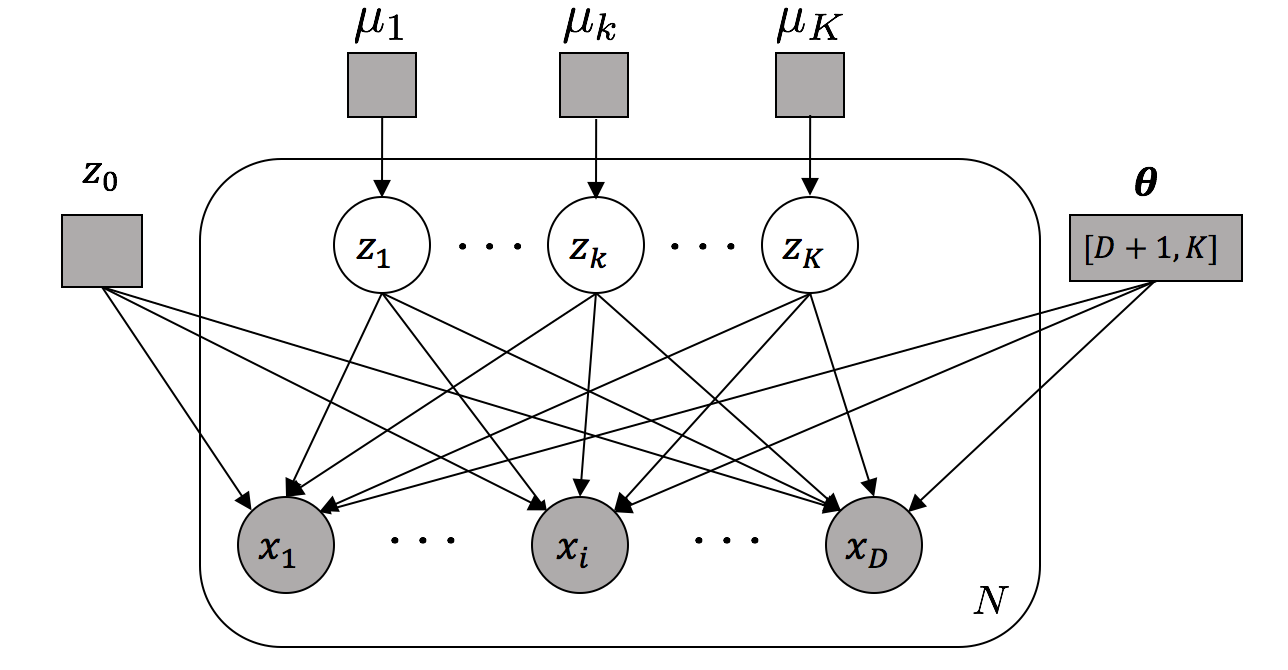
\includegraphics[height=1.2in]{NoisyORmodel.png}
\caption{\small 
\textsc{noisy-or} model in plate notations.}
\label{fig:nor}
\vskip -1em
\end{figure}



\textsc{noisy-or} is a bipartite directed graph modeling the dependencies among binary observations. 
The structure is shown in Fig.~\ref{fig:nor}, where $\bx \in \{0, 1\}^D$ represents the observed $D$-dimensional data, $\bz \in \{0, 1\}^{K+1}$ are the latent variables (with $z_0 =1$). %and $\btheta$ are the model parameters. 
The model defines the distribution
\begin{align}
     p(\bx, \bz) = \prod_{i=1}^D p(x_i|\bz) \prod_{k=0}^K p(z_k)
\label{eq: joint nor}
\end{align}
where $p(x_i|\bz)$ and $p(z_k)$ are Bernoulli distributions. In particular,
\begin{align}
    p(x_i=0|\bz) = (1-p_{i0})\prod_{k=1}^K (1-p_{ik})^{z_k}
\end{align}
where $p_{ik}=p(x_i=1|z_k=1)$. Redefining $\theta_{ik} = -\log (1-p_{ik})$, we have 
\begin{align}
    p(x_i=0|\bz) = e^{-\theta_{i0} - \sum_{k=1}^K \theta_{ik}z_k} = e^{-\btheta_i^T\bz}
\end{align}
where we slightly abuse the notation on $\btheta_i=\{\theta_{i0}, \theta_{i1}, \ldots, \theta_{iK}\}$ and $\bz=\{1, z_1, z_2, \ldots, z_K\}$.  In more compact form, we have
\begin{align}
    p(x_i|\bz) = p(x_i=1|\bz)^{x_i}p(x_i=0|\bz)^{1-x_i}.
\end{align}
where $x_i$ takes value of either 0 or 1.

The form of the likelihood of positive observation $ p(x_i=1|\bz)$ makes it intractable for computing its expectation of logarithm, even when the posterior is approximated in factorized form.

%\subsection{Variational bound via conjugate dual}
\subsection{Conjugate Dual Inference}

The conjugate dual for approximating $p(x_i=1|\bz)$ of \textsc{noisy-or} model was first introduced in~\citep{jaakkola1999variational}, where an approximate upper-bound of likelihood is:
\begin{align}
    p(x_i=1|\bz) & =e^{\log (1-e^{-a_i})} = e^{f(a_i)} \nonumber \\
   &  \leq e^{\psi_i a_i - g(\psi_i)} = \tp_(x_i=1|\bz, \psi_i) 
\label{eq:positiveUB}    
\end{align}
Here $f(a_i)$ is a concave function with $a_i = \btheta_i^T\bz$, $\psi_i$ is a variational parameter associated with $a_i$, and $g(\cdot)$ is the conjugate dual function of $f(\cdot)$. For $f(s) = \log(1-e^{-s})$, we have
\begin{equation}
g(t)  =  -t\log t + (t+1)\log (t+1)
\end{equation}
The detailed derivation can be found in~\citep{jaakkola1999variational}.


The resulting upper-bound $\log \tp(x_i=1|\bz, \psi_i)$ has an appealing property that it is linear in $a_i$ (hence, $\bz)$. Thus after applying the Bayes rule, we achieve a factorized (variational) posterior distribution
\begin{align}
    q(\bz|\bx, \bpsi)  \propto 
     &\prod_{i: x_i =1}^D\tp(x_i=1|\bz, \psi_i) \cdot \nonumber \\
     &\prod_{i: x_i=0}^Dp(x_i=0|\bz)\prod_{k=0}^K p(z_k)
\label{eq: lvi posterior}
\end{align}


Note that we only use the upper-bound for positive observations where $x_i=1$. For negative observations, we use the true likelihood.  After re-organizing the terms, we observe that
\begin{align}
    q(\bz|\bx, \bpsi) = \prod_{k=1}^K q(z_k |\bx, \bpsi)
\end{align}
Namely, the variational posterior factorizes. And each factor is
\begin{align}
    \medmath{q(z_k=1 |\bx, \bpsi) = 
    \sigma\left(\sum_{i:x_i=1}\psi_i\theta_{ik} - \sum_{i:x_i=0}\theta_{ik} + \log \frac{\mu_k}{1-\mu_k}\right)}
\label{eq:factorizedposterior}
\end{align}
where $\sigma(\cdot)$ is the sigmoid function and $\mu_k$ is the parameter of prior distribution $\mu_k = p(z_k=1)$. The detailed derivation can be found in supplementary material.   

Moreover, computing the expectation of variational upper-bound $\tp(x_i=1|\bz, \psi_i)$ with respect to the factorized (variational) posterior distribution $q(\bz|\bx, \bpsi)$ is trivial. And the gradients can be computed directly without sampling.
Hence we take $\tp(x_i=1|\bz, \psi_i)$ as the approximation to $p(x_i=1|\bz)$. 
Similarly, the likelihood conjugate lower-bound can be applied for variational inference. Interested readers could refer to \citep{jaakkola1999variational, vsingliar2006noisy}.

The conjugate dual inference (CDI) choose the best $\psi_i$ to achieve the tightest upper-bound
%\begin{equation}
%\psi_i^* = \arg\min_{\psi_i} \{\psi_ia_i - g(\psi_i)\}
%\label{eqTightBound}
%\end{equation}
\begin{align}
\psi_i^* & = \arg\min_{\psi_i} \{\tp(x_i=1)\} \nonumber\\
& = \arg\min_{\psi_i} \{\mathbb{E}_{p(\bz)}[\tp(x_i=1|\bz, \psi_i)]\}
\label{eqTightBound}
\end{align}

%\subsubsection{Variational Lower-bound}
%Similarly, the variational lower-bound is designed as:
%\begin{align}
%    \medmath{ p(x_i=1|\bz) = e^{f(a_i)} \geq e^{\bpsi_i^T f(\bu_i)} = \tp_l(x_i=1|\bz, \bpsi_i)}
%\end{align}
%where $\bpsi_i$ is a $K$-dimensional vector summing to $1$, and $\bu_i = \frac{\btheta \circ \bz}{\bpsi_i}$. The detailed derivation can be found in \citep{jaakkola1999variational}. Traditionally, we choose the best $\bpsi_i$ as 
%\begin{equation}
%    \bpsi^* = \arg\max_{\bpsi}\big\{\bpsi_i^T f(\bu_i)\big\}
%\end{equation}
%\begin{align}
%    \bpsi_i^* & = \arg\max_{\bpsi_i}\{\tp_l(x_i=1)\} \nonumber \\
%    & = \arg\max_{\bpsi_i} \{\mathbb{E}_{p(\bz)}[\tp_l(x_i=1|\bz, \bpsi_i)]\}
%\end{align}

However, in the next section, we will show that we can choose $\psi_i^*$ differently, leading to a different type of inference technique.
%we will show that we can use the upper-bound to select the form of variational distribution, and choose $\psi_i^*$ differently, leading to a different type of inference technique.

\subsection{Stochastic Variational Inference}
Recently, SVI has been proposed for (hierarchical) \textsc{noisy-or} model \citep{jivariational}. Similar to CDI, the conjugate lower-bound in \citep{jaakkola1999variational, vsingliar2006noisy} is applied to approximate the positive likelihood for its tractability of taking expectation. 
Different from CDI, where the variational posterior is constructed as eq.~(\ref{eqTightBound}), the parameters of variational posterior are treated as free-parameters and optimized directly. In other words, two sets of variational parameters are introduced:
\begin{itemize}
\setlength\itemsep{0em}
    \item[-] $\bpsi$: variational parameters introduced by the conjugate bound (eq. (\ref{eq:positiveUB})).
    \item[-] $\bphi$: parameters of variational posterior distribution $q(\bz|\bx; \bphi) = \prod_{k=1}^K q(z_k|\bx; \bphi)$.
\end{itemize}
Comparing to CDI, the unconstrained posterior gives higher inference capacity. 
Meanwhile, SVI can handle large-scale datasets and converges faster by taking mini-batches while CDI considers the whole batch during learning. 
%\todo{Not sure why whole batch}


\subsection{Amortized Variational Inference}
\label{sec: avi}
Under the auto-encoding variational Bayes framework~\citep{kingma2013auto}, AVI uses global parameters to predict the parameters of approximate posterior distribution directly. 
For instance,~\citep{kingma2013auto} predicts the parameters $\bphi$ of $\pqn$ as $\bphi = f(\bx^{(n)}; \blambda)$. Here, $\blambda$ is the global trainable parameter, which is shared across all $\bx^{(n)}$, $n=1, \cdots, N$. As a special case, $f(\cdot)$ can be a neural network and $\bphi = \textsc{mlp}(\bx; \blambda)$. 

The expectation of log-likelihood requires sampling the latent variable $\bz \sim \pqx$. However, the gradients cannot be back-propagated though stochastic random variable $\bz$. Hence for certain types of distributions $\pqx$, the reparametrization trick can be applied to reparameterize the random variable $\bz$ using a differentiable function (such as neural network) $\bz=g_{\blambda}(\bx, \mathbf{\epsilon})$, where $\mathbf{\epsilon}\sim p(\mathbf{\epsilon})$ (a known and easily sampled distribution). Then the expected log-likelihood can be rewritten as
\begin{align}
    \mathbb{E}_{\pqx}[\log p(\bx|\bz)] = \mathbb{E}_{p(\mathbf{\epsilon})}\big[\log p \left(\bx| g_{\blambda}(\bx, \mathbf{\epsilon})\right)\big]
\end{align}
which can then be computed with Monte Carlo sampling from $p(\epsilon)$.

AVI utilizes the advantages of deep neural networks as inference model without explicitly deriving complex conjugate dual functions for likelihoods, and has the power of approximating posterior flexibly. However, when there is not enough training data, the inference model might  overfit and leads to a large variance in estimating the generative model. We will introduce our method in the next section to tackle this problem.


%\subsection{Amortized Stochastic Variational Inference}
%Amortized stochastic variational inference (ASVI) can be considered as a variant of SVI. Instead of learning local parameters $\bpsi$ and $\blambda$ as free-parameters, amortization can be applied:
%\begin{align}
%    \bpsi = \textsc{mlp}(\bx; \blambda_1)
%\end{align}
%\begin{align}
%    \bphi = \textsc{mlp}(\bx; \blambda_2)
%\end{align}
%Comparing to AVI, ASVI uses a tractable approximation of ELBO and avoids the cost Monte-Carlo sampling. However, optimizing the approximation of ELBO can lead to poor performance, which will be shown in our experiments. 


